\title{Incorporating Weighted Clustering in 3D Gesture Recognition}
\author{
        John Hiesey \\
        jhiesey@cs.stanford.edu
        \and
        Clayton Mellina \\
        cmellina@cs.stanford.edu
        \and
        Zavain Dar \\
        zdar@cs.stanford.edu
}
\date{\today}

\documentclass[11pt]{article}
\usepackage[margin=0.75in]{geometry}
\usepackage{amsfonts}
\usepackage{graphicx}
\usepackage{indentfirst}
\usepackage{wrapfig}

\begin{document}
\maketitle


\section{Introduction}
We expand and improve upon the Hidden Markov Model algorithm (KHMM) presented in Klingmann [1] to improve identification of 3d gestures on mobile devices.  Specifically, we extend the algorithm to include a a weighted probability measure for clustering ``fit", as well as expand our feature space to use gyroscope information, which is available on most mobile devices today.  This gives nontrivial gains in both robustness and accuracy in 3d gesture recognition over Klingmann's initial implementation.

We alter KHMM's clustering assumptions.  Specifically, we address the implicit assumption that clustering centroids remain uniform across gesture types.  By assigning to each gesture type a unique set of centroids we make significant and immediate gains.  We derive two alternative algorithms to test our hypotheses, denoting them Cluster-Matching-HMM and Cluster-Matching.  

There are a variety of reasons why we use gyroscope information. Firstly, gyroscope data is additional information that is useful for identifying gestures, especially considering that slight variations in the device's orientation from gesture to gesture will affect accelerometer readings. These variations, however, can be corrected for with judicious use of gyroscope data. We hypothesize that a machine learning algorithm will be capable of utilizing the data to effectively make these corrections, thereby resulting in better orientation invariance.  Secondly, if we wish to use 3d gestures as an input modality for mobile devices, inclusion of gyroscope information offers opportunities for greater expressiveness. Gestures can now include and be differentiated by orientation changes.

On a pragmatic note, we develop and test on the iPhone platform, although our solutions have general applicability, and an available Matlab implementation. The iPhone is chosen amongst our team as two of our members have previous iPhone development experience.  
% \pagebreak

\section{Data}
As with any learning algorithm we require to have some data available.  We use Apple's iPhone and xSensor application to record, train and test our various algorithms.  For each training example for any gesture type xSensor returns to us an ordered series of vectors in $\mathbb{R}^n$ containing instantaneous acceleration and gyroscope data sampled at 32 hz.  For the most part we normalize each training example by scaling each vector in the training example by $\frac{n}{\sum_n{\parallel x_n \parallel}}$, where the training example consists of $n$ instantaneous feature vectors.  


\section{Algorithms}
We now discuss the three main algorithms that we examine and analyze, starting first with Klingmann's baseline KHMM, followed by our Cluster-Matching-HMM and Cluster-Matching alterations.  

\subsection{KHMM}


KHMM uses k-means clustering to discretize the space of real vectors followed by training one Hidden Markov Model for each gesture type.  The intuition behind this can be thought of as follows: the clustering across all gesture types serves mainly to project each data vector which is in $ \mathbb{R}^n $ (where there are $n$ features) to $\mathbb{Z^{+}}$.  Concretely, this discretizes the data uniformly regardless of what gesture type it belongs to.  Following the discretization KHMM then trains a Hidden Markov Model of the discretized training sets for each gesture type.
\\
\\
Formally we describe the algorithm as follows:

	\subsubsection{Clustering}
		For all training examples across all gesture types, running k-means on all of the training data simultaneously defines a single clustering function $f: \mathbb{R}^n \rightarrow \mathbb{Z^{+}}$. 
	\subsubsection{Hidden Markov Model}
		For each set of training examples for each gesture type, train a Hidden Markov Model.  Namely in this stage, for each gesture type $g$, we generate a function $h_g: (\mathbb{Z^{+}}^k) \rightarrow \mathbb{R}_{[0,1]}$  by the Hidden Markov Model process:
$HMM: (\mathbb{Z^{+}}^k)^t \rightarrow h_g$, where each training example consists of $k$ instantaneous data points and there are $t$ training examples for gesture type g.  
	\subsubsection{Classification Procedure}
		To classify an unknown gesture example, which exists in $(\mathbb{R}^n)^k$, we first transform it to its discretized version, namely $f(\mathbb{R}^n)^k$ and then for each gesture type $g$, apply $h_g((f(\mathbb{R}^n))^k)$ and classify the example according to the $g�$ were $h_g�$ returns maximum probability. 
		
		
\subsection{Cluster-Matching-HMM}

The motivation for Cluster-Matching-HMM derives from the realization that in the clustering step KHMM applies the same centroids to each training example regardless of what gesture type it belongs to.  We hypothesize that different gesture types have vastly different vector features score (i.e. lie in different subspaces of $\mathbb{R}^n$) and thus we might gain information by clustering each gesture type independently and then training an HMM for each clustered training type.  In the classification step we then classify over each clustering and each corresponding HMM.  Moreover we weight the resulting HMM probabilities according to how well the training example ``fits" in the the assigned cluster.  
\\
\\
Formally we describe the algorithm as follows:

	\subsubsection{Clustering}
		For each gesture type $g$ across all training examples, running k-means on all of the training data from for one gesture only defines a clustering function $f_g: \mathbb{R}^n \rightarrow \mathbb{Z^{+}}$ for each gesture type.
	\subsubsection{Hidden Markov Model}
		For each set of training examples for each gesture type, train a Hidden Markov Model.  Namely in this set we generate a function $h_g: (\mathbb{Z^{+}}^k) \rightarrow \mathbb{R}_{[0,1]}$ by the Hidden Markov Model process: 
		$HMM: (\mathbb{Z^{+}}^k)^t \rightarrow h_g$, where each training example consists of $k$ instantaneous data points and there are $t$ training examples for gesture type $g$.  

	\subsubsection{Classification Procedure}
	To classify a new example, which exists in $(\mathbb{R}^n)^k$, we first transform, for each gesture type $g$, the training example to it�s discretized version, namely $f_g(\mathbb{R}^n)^k$ and then apply $h_g((f_g(\mathbb{R}^n))^k)$.  Finally, we classify the example according to the $g'$ where $h_{g^{'}} * p((f_{g^{'}})^k)$ returns the maximum value.  Here $p$ is a ``fittness value" of how well the training example fit into the given clustering.  Namely we used an aggregate sum of the distances of the training vectors to their respective assigned centroids.  Thus not only does each gesture type receive its own HMM but also its own clustering.  
	

	\subsection{Cluster-Matching}

Motivated by the effectiveness\footnote{See results.} of Cluster-Matching-HMM we define Cluster-Matching to naively cluster the training examples for specific gesture types.  Then, when classifying, we assign an unknown gesture type to the gesture clustering to which it best fits.  
\\
\\
Formally we describe the algorithm as follows:

		\subsubsection{Clustering}
		For each gesture type $g$ across all training examples, k-means defines a clustering function $f_g: \mathbb{R}^n \rightarrow \mathbb{Z^{+}}$.

		 \subsubsection{Classification Procedure}
 		For all $g$, compute $p((f_g(\mathbb{R}^n))^k)$.  Return $g$ that returns minimum value.  


\section{Results}\label{results}

We tested our algorithms\footnote{All code available at https://github.com/jhiesey/GestureRecognizer} on six datasets: circles (with the phone held relatively flat), triangles (with the phone held similarly), bowling motions, flicking the phone upward, and flicking up and to the right.  The last set, used only in a few tests, consisted of squares.  These datasets all include gestures of deliberately variable quality: some are carefully controlled, and others less so.

\begin{center}
\begin{tabular}{ | l | l | l | l | l | }
  \hline
  Normalization & Features & Gestures Types & Algorithms & Accuracy \\ \hline
  Yes	&	Both  &	All & Cluster-Matching-HMM (10) &	94.6\% \\ \hline
  Yes	&	Both	&	All & KHMM  &	89.6\% \\ \hline
  No	&	Both	&	All & KHMM  &	88.4\% \\ \hline
  Yes	&	Accel &	All & Cluster-Matching-HMM (10) &	92.0\% \\ \hline
  Yes	&	Accel &	All &	KHMM & 84.2\% \\ \hline
  Yes	&	Gyro  &	All & Cluster-Matching-HMM (10) & 92.3\% \\ \hline
  Yes	&	Gyro  &	All & KHMM &  89.7\% \\ \hline
  Yes	&	Both	&	All &	Cluster-Matching (10) &  96.7\% \\ \hline
  Yes	&	Both	&	All &	Cluster-Matching (20) &  97.9\% \\ \hline
  Yes	&	Both  &	All &	Cluster-Matching (40) & 	98.4\% \\ \hline
  No	&	Both	&	All &	Cluster-Matching (40) & 	98.4\% \\ \hline
  Yes	&	Both	& Squares and Triangles &	Cluster-Matching (10) & 	100\% \\ \hline
  Yes	&	Both	& Circles and Reversed-circles  &	Cluster-Matching (10) & 	Chance \\ \hline
  Yes	&	Both	& Circles and Reversed-circles  &	Cluster-Matching-HMM (10) &	72.0\% \\ \hline
  Yes	&	Both  & Circles and Reversed-circles  &	Cluster-Matching-HMM (20) & 88.8\% \\
  \hline
\end{tabular}
\end{center}

\subsection{Choice of features}
In general, the highest accuracy is achieved when using both accelerometer
and gyroscope data, followed by gyroscope data only, followed by accelerometer data only.

For example, using Cluster-Matching-HMM, both accelerometer and gyroscope data together
achieves 94.6\% on all gesture types, followed by gyroscope data only at 92.3\%, and
accelerometer data only at 92.0\%.  The same general pattern is evident in the KHMM
data as well.

As we could not find any examples of using gyroscope data for gesture recognition
in the literature, this seems to be unique way of improving gesture recognition
accuracy.

\subsection{Clustering approach}
Our initial approach of clustering on all training data together
worked reasonably well.  When running on all 5 sample gestures and
with the HMM enabled, we got an an accuracy of 89.6\%.

However, on the same data, our Cluster-Matching algorithm combined with
an HMM reaches 94.6\% accuracy.  We also observed similar improvements with
other examples, as seen in the data.

\subsection{HMM}
Although we found a few examples where the Cluster-Matching algorithm
benefits from using a Hidden Markov Model, in most real-world examples
there is little benefit.  When running on all of the training data,
we found that adding the HMM actually decreased accuracy slightly,
from 96.7\% to 94.6\%, which may be due to random fluctuations.

However, when comparing the data for circles to our contrived data
set consisting of the first and second halves of each circle switched,
then using an HMM with alphabet size of 20 improved the results from chance
to 88.8\%.  Unfortunately we could not get such dramatic improvements with
any non contrived data.

\subsection{Number of symbols}
Increasing the number of symbols in the HMM's alphabet improves accuracy
up to a point, but at the cost of a decrease in performance.


\begin{wrapfigure}{r}{0.5\textwidth}
\center
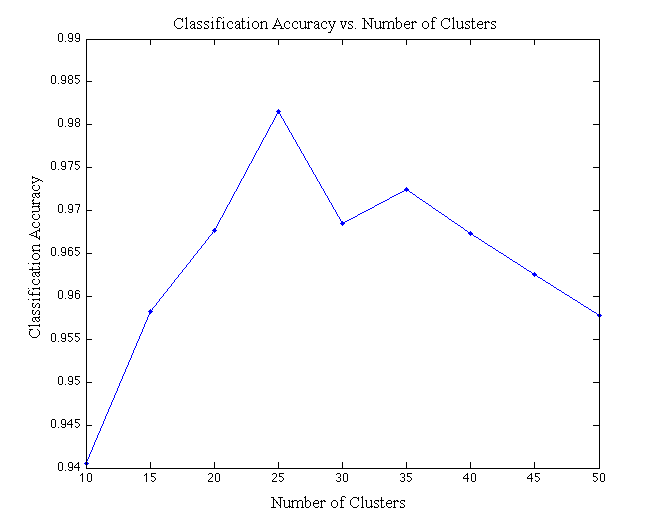
\includegraphics[scale=0.5]{accuracy_vs_num_clusters.png}
\caption{Classification accuracy of Cluster-Matching-HMM for 6 gestures}
\label{fig:alphabetsize}
\end{wrapfigure}

% For example, on the five KHMM gestures, increasing the alphabet size
% from 10 to 40 improves the accuracy from 96.7\% to 98.4\%.  On the contrived
% circle data, the improvement was much larger, from 72.0\% to 88.8\%.

As shown in Figure~\ref{fig:alphabetsize}, the optimum accuracy is achieved
at an alphabet size of around 25 symbols, with gradually decreasing accuracy
outside of that range.

\subsection{Normalization}
In general, our normalization makes only a small difference.  With the
KHMM algorithm we saw an improvement of less than 1.5\% in accuracy,
and we saw no detectable difference using Cluster-Matching.


\section{Future Research}
We see a variety of promising avenues for the future development of Cluster-Matching. More work needs to be done to assess the scalability of our method, although the outlook is promising. Current literature on accelerometer-based gesture recognition usually reports classification results for 4 to 8 gesture types. We believe that our method has the potential to scale to more gesture types given our current results. Our technique currently incorporates centroid-distance and HMM log-likelihood scores heuristically by simply multiplying them before classifying. It is likely that a more principled method of combining centroid-distance and HMM loglikelihood - one possibly incorporating the data itself - will yield better results. This becomes especially important for gestures in which one component of the classifier performs significantly better than the other. Lastly, future work should address the possibility of using Cluster-Matching for automated segmentation of continuous accelerometer and gyroscope data. Current proposals use only heuristic methods and do not incorporate the trained gesture classifier, e.g. Prekopcs�k demonstrates the feasibility of using a speed threshold to detect the onset of a gesture. HMMs do not provide an obvious means by which to use them for segmentation, as they will readily assign log-likelihoods to sequences of any length [3]. We suspect that Cluster-Matching can be computed over a sliding window on the data stream, providing a means by which to determine when a sequence of samples is being fit well by a subset of the clusters of one of the gesture cluster-sets.

\section{Conclusions}\label{conclusions}
We thus show non trivial gains in accuracy with resect to our baseline classifier KHMM.  These gains are accrued not only through the collection of a new set of features using gyroscope data, but also through our novel algorithms Cluster-Matching-HMM and Cluster-Matching.  Interestingly enough it appears that erven though we are classifying sequential data, simply assigning cluster fitness scores to all the vectors in a gesture example, regardless of sequential order, returns the most accurate classifiers.  In fact, the only times when this is not the case is when we synthetically manipulate the data files to purposely break our Cluster-Matching classifier.  However, we could not mimic this ``break case" using actual gesture data.  We are thus confident in the ability of Cluster-Matching to accurately classify real human gestures.  Regardless, we hope to have pushed forward the study and field of gesture recognition; not only by presenting classifiers with high accuracy, but also through the presentation of a new cluster based paradigm of classifiers.  

  \begin{thebibliography}{1}
  
  \bibitem{orig} Klingmann, Marco. {\em Accelerometer-Based Gesture Recognition with the iPhone}. Masters Thesis, Goldsmith University of London. 2009.
  
  \bibitem{svm} Wu, Jiahui and Pan, Gang and Zhang, Daqing and Qi, Guande and Li, Shijian. {\em Gesture Recognition with a 3-D Accelerometer}.  2009.

  \bibitem{seg}  Zolt�n Prekopcs�k {\em Accelerometer Based Real-Time Gesture Recognition}. 2008.
  


  \end{thebibliography}

\end{document}